\section{Introduction}
Motif searching is an important step in the detection of rare events
occurring in a set of DNA or protein sequences. The Planted Motif Search (PMS)
problem, also known as the $(l,d)$-motif problem, has been introduced in \cite{Pev00} with the aim of detecting motifs and significant
conserved regions in a set of DNA or protein sequences. PMS receives as
input $n$ biological sequences and two integers $\ell$ and $d$.
It returns all possible biological sequences $M$ of length $\ell$
such that $M$ occurs in each of the input strings, and each
occurrence differs from $M$ in at most $d$ positions. Any such
$M$ is called a motif. Given two $\ell$-mers, the number of positions in which
they differ is called their Hamming distance.

Buhler and Tompa \cite{BuTo01} have employed PMS algorithms to find known transcriptional regulatory elements upstream of several eukaryotic genes. In particular, they have used orthologous sequences from different organisms upstream of four different genes: preproinsulin, dihydrofolate reductase (DHFR), metallothioneins, and c-fos. These sequences are known to contain binding sites for specific transcription factors. Their algorithm successfully identified the experimentally determined transcription factor binding sites. 
They have also employed their algorithm to solve the ribosome binding site
problem for various prokaryotes. Eskin and Pevzner \cite{EsPe02} used PMS
algorithms to find composite regulatory patterns using their PMS algorithm
called MITRA. They have employed the upstream regions involved in purine
metabolism from three {\em Pyrococcus} genomes. They have also tested their
algorithm on four sets of {\em S.cerevisiae} genes which are regulated by two
transcription factors such that the transcription factor binding sites occur
near each other. Price, et al. \cite{PRP03}  have employed their
PatternBranching PMS technique to find motifs on a sample containing CRP binding
sites in {\em E.coli}, upstream regions of many organisms of the eukaryotic
genes:
preproinsulin, DHFR, metallothionein, \& c-fos, and a sample of yeast promoter regions.

A problem that is very similar to $(\ell,d)$ motif search is the Closest Substring problem. The
Closest Substring problem is essentially the PMS problem where the aim is to
find the smallest $d$ for which there exists at least one motif. These two problems
have applications in PCR primer design, genetic probe design, discovering
potential drug targets, antisense drug design, finding unbiased consensus of a
protein family, creating diagnostic probes and motif finding (see e.g.,
\cite{LLM+99}). Therefore, the development of efficient algorithms for solving
the PMS problem constitute an active interest in biology and bioinformatics.

In a practical scenario, instances of the motif may not appear in all of
the input strings. This has led to the introduction of a more general
formulation of the problem, called quorum PMS (qPMS). In qPMS we are interested
in motifs that appear in at least $q$ percent of the $n$ input strings.
Therefore, when $q=100\%$ the qPMS problem is the same as PMS.

The Closest Substring problem is NP-Hard \cite{LLM+99}. The Closest Substring
problem can be solved by a linear number of calls to PMS. Therefore,
there is a polynomial time reduction from Closest Substring to PMS, which
means that the PMS problem is also NP-Hard. Because of this, all known exact
algorithms have an exponential runtime in the worst case.
Thus, it is important to develop efficient algorithms in practice. 

The practical performance of PMS algorithms is
typically evaluated on datasets generated as follows (see \cite{Pev00,DBR07}):
20 DNA/protein strings of length 600 are generated according to the
independent identically distributed (i.i.d.) model. Then, a random
motif ($\ell$-mer) $M$ is similarly generated and ``planted'' at a random
location in each input string (or in $q\%$ of the input strings for qPMS).
Every planted instance of the motif is mutated in exactly $d$ positions.


\begin{definition}
An $(\ell,d)$ instance is defined to
be a {\bf challenging instance} if $d$ is the largest integer for which the
expected number of motifs of length $\ell$ that would occur in
the input by random chance does not exceed a constant (500 in this thesis, same
as in \cite{NRPMS14}).
\end{definition}

Intuitively, the more we increase $d$, the more we increase the search space.
However, if we increase $d$ too much, we find many motifs just by
random chance (spurious motifs). Hence, the challenging instances for PMS on
DNA data, according to the above definition, are $(13,4)$, $(15,5)$, $(17,6)$,
$(19,7)$, $(21,8)$, $(23,9)$, $(25,10)$, $(26,11)$, $(28,12)$, $(30,13)$, etc.

A PMS algorithm can be exact or approximate. An exact algorithm finds all
the existing motifs. Note that in this chapter we only address exact algorithms. 
Namely, we will discuss two algorithms: PMS8 \cite{NRPMS14}
and its successor qPMS9 \cite{NRPMS15}.

Given a tuple of $\ell$-mers, the set of $\ell$-mers that have a Hamming
Distance of no more than $d$ from any $\ell$-mer in the tuple is called the
{\em common $d$-neighborhood} of the tuple.

There are many PMS algorithms in the literature. Most of the exact PMS
 algorithms use a combination of two fundamental techniques. One technique is sample driven and the other
technique is pattern driven. In the sample driven stage, the algorithm selects
a tuple of $\ell$-mers coming from distinct input strings.  Then, in the pattern driven stage,
the algorithm generates the common $d$-neighborhood of the $\ell$-mers in the tuple.
Each neighbor becomes a motif candidate. The size of the tuple
is usually fixed to a value such as 1 (see e.g. \cite{RBH05,DBR07,RD11}), 2 (see
e.g.
\cite{YHZG12}), 3 (see e.g. \cite{T14,DRK11,BSR12,DRD12}) or $n$ (see e.g.
\cite{Pev00,IA14}). The algorithms described in this chapter, PMS8
\cite{NRPMS14} and qPMS9 \cite{NRPMS15}, utilize a variable tuple size, which
adapts to the problem instance under consideration. 


For tuples of size 3, qPMS7 \cite{DRD12} computes neighborhoods by using an
Integer Linear Programming (ILP) formulation. A large number of ILP
instances are solved and stored in a table, as a preprocessing step.
This table is then repeatedly looked up to identify common neighbors of three $l$-mers. This preprocessing step takes a considerable amount of time
and the look up table requires a large amount of memory. 

In this chapter
we state and prove necessary and sufficient conditions for $3$ $l$-mers to have a
common neighbor, therefore removing the requirement for a large look up table.
These conditions generalize to necessary (but not sufficient) conditions for $4$
or more $\ell$-mers to have a common neighborhood. These conditions are
used as pruning techniques that form the basis for the efficiency of PMS8,
along with several speedup techniques. 

We have used PMS8 as the basis for the
qPMS9 algorithm. The qPMS9 algorithm extends PMS8 in several ways. First, qPMS9
introduces a string reordering procedure which significantly increases
performance by allowing for better pruning of the search space. Second, qPMS9 adds support for
solving the qPMS problem, which was lacking in PMS8.


The first algorithm to solve the challenging DNA instance  $(23,9)$ has
been the qPMS7 algorithm \cite{DRD12}. The algorithm in \cite{DeM11}
can solve instances with relatively large $l$ (up to $48$) provided that $d$ is at most $l/4$. However, most of the well known
challenging instances have $d>l/4$. PairMotif \cite{YHZG12} can solve instances
with larger $l$, such as $(27,9)$ or $(30,9)$, but these are significantly less
challenging than $(23,9)$.

The first algorithm to solve $(25,10)$, in a reasonable amount of time (no more
than two days using commodity processors) has been TraverStringRef \cite{T14}. The TraverStringRef
algorithm \cite{T14} is an algorithm for the qPMS problem, based on the earlier
qPMS7 \cite{DRD12} algorithm. PMS8 can solve DNA instances (25,10), on a single core
machine, and (26,11) on a multi-core machine. Its successor, qPMS9,
can solve $(28,12)$ and $(30,13)$ on a single core machine. 
Several of these algorithms are compared with PMS8
and qPMS9 in section \ref{sec_pms_results}.

 

\section{Methods}

We start by defining the PMS and qPMS problems more formally. A string of
length $\ell$ is called an $\ell$-mer. Given two $\ell$-mers $u$ and $v$, the
number of positions where the two $\ell$-mers differ is called their Hamming
distance and is denoted as $Hd(u,v)$. 
If $T$ is a string,  $T[i..j]$ denotes the substring of $T$ starting at
position $i$ and ending at position $j$.

\begin{problem}
{\bf PMS}: Given $n$ sequences $s_1, s_2, \ldots, s_n$,
over an alphabet $\Sigma$, and two integers $\ell$ and $d$, identify all
$\ell$-mers $M$, such that $M \in \Sigma^l$ and $\forall i,1\leq i\leq
n$, $\exists j_i, 1\leq j_i\leq |s_i|-l+1$, s. t.
$Hd(M,s_i[j_i..j_i+l-1])\leq d$.
\end{problem}

\begin{problem}
{\bf qPMS}: same as the PMS problem, however the motif should
appear in at least $q\%$ of the strings, instead of all of them. PMS is a special case of qPMS for which $q=100\%$.
\end{problem}

Another useful notion is that of a $d$-neighborhood. Given a
tuple of $\ell$-mers $T=(t_1,t_2,\ldots,t_s)$, the common $d$-neighborhood of
$T$ includes all the $\ell$-mers $r$ such that $Hd(r,t_i)\leq d$,
$\forall 1\leq i\leq s$.

We now define the consensus $\ell$-mer and the
consensus total distance for a tuple of $\ell$-mers. Given a tuple of
$\ell$-mers $T=(t_1, \ldots, t_k)$ the {\bf consensus $\ell$-mer}
of $T$ is an $\ell$-mer $u$ where $u[i]$ is the most common character among
$(t_1[i], t_2[i], \ldots, t_k[i])$ for each $1\leq i \leq \ell$. If the
consensus $\ell$-mer for $T$ is $p$ then the {\bf consensus total distance} of
$T$ is defined as $Cd(T)=\sum_{u\in T}Hd(u,p)$. While the consensus string is generally not a motif, the
consensus total distance provides a lower bound on the total distance between
any motif and a tuple of $\ell$-mers, as we show in section
\ref{sec_pms_pruning}.

As indicated previously, most of the motif search algorithms combine a sample
driven approach with a pattern driven approach. In the sample driven part, tuples of $\ell$-mers $(t_1,
t_2, \ldots, t_k)$ are generated, where $t_i$ is an $\ell$-mer in $S_i$. Then,
in the pattern driven part, for each tuple, its common $d$-neighborhood is
generated. Every $\ell$-mer in the neighborhood is  a candidate motif. In
PMS8 and qPMS9, the tuple size $k$ is variable.
By default, a good value for $k$ is estimated heuristically (see
\cite{NRPMS14}) based on the input parameters, or $k$ can be user specified.

\subsection{Generating Tuples of $\ell$-mers}

In the sample driven part of PMS8 we generate tuples $T=(t_1, t_2,
\ldots, t_k)$, where $t_i$ is an $\ell$-mer from string $s_i$, $\forall i=1..k$, based
on the following principles.
First, if $T$ has a common $d$-neighbor, then every subset of $T$ has a
common $d$-neighbor.
Second, there has to be at least one $\ell$-mer $u$ in
each of the remaining strings $s_{k+1}, s_{k+2}, \ldots, s_n$ such that $T \cup
\{u\}$ has a common $d$-neighbor. We call such $\ell$-mers $u$
``alive'' with respect to tuple $T$.


As we add $\ell$-mers to $T$, we update the alive $\ell$-mers in the remaining
strings. Based on the  number of alive $\ell$-mers, in PMS8 we reorder the
remaining strings increasingly. This is a heuristic that speeds up the search
because the first $\ell$-mers in the tuple are the most expensive so
we want as few combinations of them as possible. However, in qPMS9 we used the
following more efficient string reorder heuristic. Let $u$ be an alive $\ell$-mer with respect to $T$. If we add $u$ to $T$, then the consensus total distance of $T$ increases.
We compute this additional distance $Cd(T\cup\{u\})-Cd(T)$. For each of the remaining strings,
we compute the minimum additional distance generated by any alive
$\ell$-mer in that string. Then we sort the strings decreasingly by the minimum additional
distance.
Therefore, we give priority to the string with the largest minimum additional
distance. 
The intuition is that larger minimum additional distance could indicate more
``diversity" among the $\ell$-mers in the tuple, which means smaller common
$d$-neighborhoods. 
If two strings have the same minimum additional distance, we give
priority to the string with fewer alive $\ell$-mers.

The tuple generation is described in
algorithm \ref{algGenTuplesPMS}. We invoke the algorithm as $GenTuples(\{\},
k, R)$ where $k$ is the desired size of the tuples and $R$ is a matrix
that contains all the $\ell$-mers in all the input strings, grouped as one row
per string. This matrix is used to keep track of alive $\ell$-mers. To
exclude tuples that cannot have a common neighbor we employ
the pruning techniques in section \ref{sec_pms_pruning}.


\commentOut{
\begin{figure}
    \centering
    \includegraphics[width=1.0\textwidth]{algGenTuples}
    \caption{This pseudocode generates tuples of $\ell$-mers that can
    potentially have common neighbors,
    for the PMS problem. \label{algGenTuplesPMS}}
\end{figure}
}

\begin{algorithm}
\SetKwInOut{Input}{Input}
\SetKwFunction{GenerateTuples}{GenerateTuples}
\SetKwFunction{ConsTotalDist}{Cd}
\SetKwFunction{GenerateNeighborhood}{GenerateNeighborhood}
\SetKwFunction{continue}{continue}

\caption{GenerateTuples$(T,k,R)$} \label{algGenTuplesPMS}
\Input{$T=(t_1,t_2,\ldots,t_i)$, current tuple of $\ell$-mers\;
\Indp\Indp $k$, desired size of the tuple\; 
           $R$, array of $n-i$ rows, where $R_j$ contains all alive
           $\ell$-mers from string $s_{i+j}$\; 
}
\KwResult{Generates tuples of size $k$, containing $\ell$-mers, that have
common neighbors, then passes these tuples to the $\GenerateNeighborhood$
function\;} \Begin{ \If {$|T|==k$}{ $\GenerateNeighborhood(T,d)$\;
\Return\;
}
outerLoop: \For {$u\in R_1$}{
$T':=T\cup \{u\}$\; 
\For{$j \leftarrow 1$ \KwTo $n-i-1$}{
$R'_{j}=\{v \in R_{j+1} | \exists\; \text{common $d$-neighborhood for}\; T' \cup
\{v\}\}$\;
\If {$|R'_j|==0$} {
\continue outerLoop\;
}
$minAdd:=\min_{v \in R'_{j}} \ConsTotalDist(T'\cup \{v\}) -
\ConsTotalDist(T')$\; 
$aliveLmers:=|s_{i+j+1}|-|R'_{j}|$\; 
$sortKey[j]:= (minAdd, -aliveLmers)$ 
}
sort $R'$ decreasingly by $sortKey$\;
\GenerateTuples$(T', k, R')$\;
}
}
\end{algorithm}


\subsection{Generating Common Neighborhoods}

For every tuple that algorithm \ref{algGenTuplesPMS} generates we want to
generate a common neighborhood. Namely, given a tuple $T=(t_1,
t_2, \ldots, t_k)$ of $\ell$-mers, we want to generate all $\ell$-mers $M$ such
that $Hd(t_i, M) \leq d, \forall i=1..k$. To do this, we traverse the tree of
all possible $\ell$-mers, starting with an empty string and adding one
character at a time. A node at depth $r$, which represents an $r$-mer, is
pruned if certain conditions are met (see section
\ref{sec_pms_pruning}). The pseudocode for neighborhood generation is given in
algorithm \ref{algGenNeighborsPMS}.

\begin{algorithm}
\SetKwInOut{Input}{Input}
\SetKwFunction{GenerateNeighborhood}{GenerateNeighborhood}
\SetKwFunction{GenerateLmers}{GenerateLMers}
\SetKwFunction{prune}{prune}
\SetKw{not}{not}

\caption{GenerateNeighborhood$(T,d)$}\label{algGenNeighborsPMS}
\Input{$T=(t_1,t_2,\ldots,t_k)$, tuple of $\ell$-mers\;
\Indp\Indp $d$, maximum distance for a common neighbor\; 
}
\KwResult{Generates all common $d$-neighbors of the $\ell$-mers in $T$\;} 
\Begin{
\For{$i \leftarrow 1$ \KwTo $|T|$}{
  $r[i]=d\;$
}
\GenerateLmers($x,0,T,r$)\;
}
\SetKwProg{myproc}{Procedure}{}{}
\myproc{\GenerateLmers{$x,p,T,r$}}{
\Input{ $x$, the current $\ell$-mer being generated\;
\Indp\Indp $p$, the current length of the $\ell$-mer being generated\;
               $T=(t_1,t_2,\ldots,t_k)$, tuple of $(\ell-p)$-mers\;
               $r[i]$, maximum distance between the (yet to
               be generated) suffix of $x$ and $t_i$, $\forall i=1..k$\; } 
\KwResult{Generates all possible suffixes of $x$ starting at
position $p$ such that the distance between the suffix of $x$ and $t_i$
does not exceed $r[i]$, $\forall i=1..k$\;} 
\eIf{$p == \ell$}{report $\ell$-mer $x$\;}{
\If{\not \prune{T,r}}{
\For{$\alpha \in \Sigma$}{
$x_p=\alpha$\;
\For{$i \leftarrow 1$ \KwTo $|T|$}{
\eIf{$t_i[0] == \alpha$}{
$r'[i]=r[i]$\;
}{
$r'[i]=r[i]-1$\;
}
$t_i'=t_i[1..|t_i|]$\;
}
\GenerateLmers{$x,p+1,T',r'$}\;
}
}
}
}
\end{algorithm}

\subsection{Pruning Conditions}
\label{sec_pms_pruning}
In this section we address the following question.
Given a tuple $T=(t_1,t_2,\ldots,t_k)$ of $\ell$-mers and a tuple
$D=(d_1,d_2,\ldots,d_k)$  of distances, is there an $\ell$-mer $M$ such that
$Hd(M,t_i)\leq d_i, \forall i=1..k$? This question appears in algorithm
\ref{algGenTuplesPMS} where $T$ is the current tuple and $D$ is an
array with all values set to $d$. The same question appears in
algorithm \ref{algGenNeighborsPMS} where $T$ is a tuple of suffixes and $D$ is an array
of remaining distances.

Two $\ell$-mers  $a$ and $b$ have a common neighbor $M$ such that $Hd(a,M)\leq
d_a$ and $Hd(b,M)\leq d_b$ if and only if $Hd(a,b)\leq d_a+d_b$.  For $3$
$l$-mers, no trivial necessary and sufficient conditions have been known up to now. We give simple
necessary and sufficient conditions for 3 $\ell$-mers to have
a common neighbor. These conditions are also necessary (but not sufficient) for
$4$ or more $\ell$-mers.

\begin{lemma}
\label{lemma_pms_total_dist}
Let $T=(t_1,t_2,\ldots,t_k)$ be a tuple of $\ell$-mers and 
$D=(d_1,d_2,\ldots,d_k)$ be a tuple of distances, and $M$ be an $\ell$-mer. If
$\sum_{i=1}^{k}Hd(M,t_i) > \sum_{i=1}^{k}d_i$ then, by the pigeonhole
principle, at least one $l$-mer $t_i$ must have $Hd(M,t_i) > d_i$. Therefore,
$M$ cannot be a common neighbor of the $l$-mers in $T$, under the given
distances.
\end{lemma}

Suppose we have a lower bound on the total distance $\sum_{i=1}^{k}Hd(M,t_i)$,
and that lower bound is independent of $M$. If that lower bound is
greater than $\sum_{i=1}^{k}d_i$ then there is no $M$ that is a common neighbor for
$T$. One such lower bound is the {\em
consensus total distance}.
To prove this, we observe an alternative definition of the consensus total
distance:

\begin{lemma}
Let $T=(t_1,t_2,\ldots,t_k)$ be a tuple of $\ell$-mers. For every $i$, the set
$t_1[i],t_2[i],..,t_k[i]$ is called the $i$-th column of $T$.
Let $m_i$ be the maximum frequency of any character in column $i$, i.e., $m_i$
is the frequency of the consensus character for column $i$.
Then the consensus total distance $Cd(T)=\sum_{i=1}^{\ell}k-m_i$.
\end{lemma}

Now consider the total distance $\sum_{i=1}^{k}Hd(M,t_i)$ between any $l$-mer
$M$ and the $l$-mers in $T$.
For any $M$, column $i$ contributes at least $k-m_i$ to the total
distance. Therefore, $\sum_{i=1}^{\ell}k-m_i$ is a lower bound for the total
distance. In other words, $Cd(T)$ is a lower bound
for the total distance for any $M$. Therefore, we have the following lemma:

\begin{lemma}
\label{lemma_consensus}
Let $T=(t_1,t_2,\ldots,t_k)$ be a tuple of $l$-mers and
$D=(d_1,d_2,\ldots d_k)$ be a tuple of non-negative integers.
There exists an $l$-mer $M$ such that $Hd(M,T_i)\leq d_i, \forall i$, only if
$Cd(T)\leq \Sigma_{i=1}^kd_i$.
\end{lemma}

We are now ready for the main theorem:

\begin{theorem}
\label{th_3sufficient}
Let $T=(t_1,t_2,t_3)$ be a tuple of three $l$-mers and $D=(d_1,d_2,d_3)$ be
a tuple of three non-negative integers. There exists an $l$-mer $M$ such that
$Hd(M,T_i)\leq d_i, \forall i, 1\leq i\leq 3$ if and only if the following conditions hold:
\begin{description}
\item[i)]  $Cd(t_i,t_j)\leq d_i+d_j, \forall i,j, 1 \leq i < j \leq 3$
\item[ii)] $Cd(T) \leq d_1+d_2+d_3$
\end{description}
\end{theorem}


\begin{proof}
The ``only if'' part follows from lemma~\ref{lemma_consensus} and from the fact
that if three $\ell$-mers have a common neighbor then any two of them must also
have a common neighbor.

For the ``if'' part we show how to
construct a common neighbor $M$ provided that the conditions hold.
We say that a column $k$ where
$t_1[k]=t_2[k]=t_3[k]$ is of type $N_0$. If $t_1[k]\neq t_2[k] = t_3[k]$ then
the column is of type $N_1$. If $t_1[k]=t_3[k]\neq t_2[k]$ then the
column is of type $N_2$ and if $t_1[k]=t_2[k]\neq t_3[k]$ then the column is of
type $N_3$. If all three characters in the column are distinct then the
column is of type $N_4$. Let $n_i, \forall i, 0\leq i \leq 4$ be
the number of columns of type $N_i$. Consider two cases:

Case 1) There exists $i, 1 \leq i \leq 3$ for which $n_i \geq d_i$. We construct
$M$ as illustrated in figure~\ref{figProofCase1}. Pick $d_i$ columns of type
$n_i$. For each chosen column $k$ set $M[k]=t_j[k]$ where $j\neq i$. For all
other columns  set $M[k]=t_i[k]$. Therefore $Cd(t_i, M) = d_i$.
For $j\neq i$ we know that $Cd(t_i,t_j)
\leq d_i+d_j$ from condition $\textbf{i)}$ (condition $\textbf{i}$ is assumed to be
true at this point because we are proving the ``if'' part).
We also know that $Cd(t_i,M)+Cd(M,t_j)\leq Cd(t_i,t_j)$ from the triangle
inequality.
It follows that $Cd(M,t_j)\leq d_j$. Since $Cd(M,t_j)=Hd(M,t_j)$ it means that
$M$ is indeed a common neighbor of the three $l$-mers.

\begin{figure}[!h]
\caption{Proof of theorem~\ref{th_3sufficient},  case 1}\label{figProofCase1}
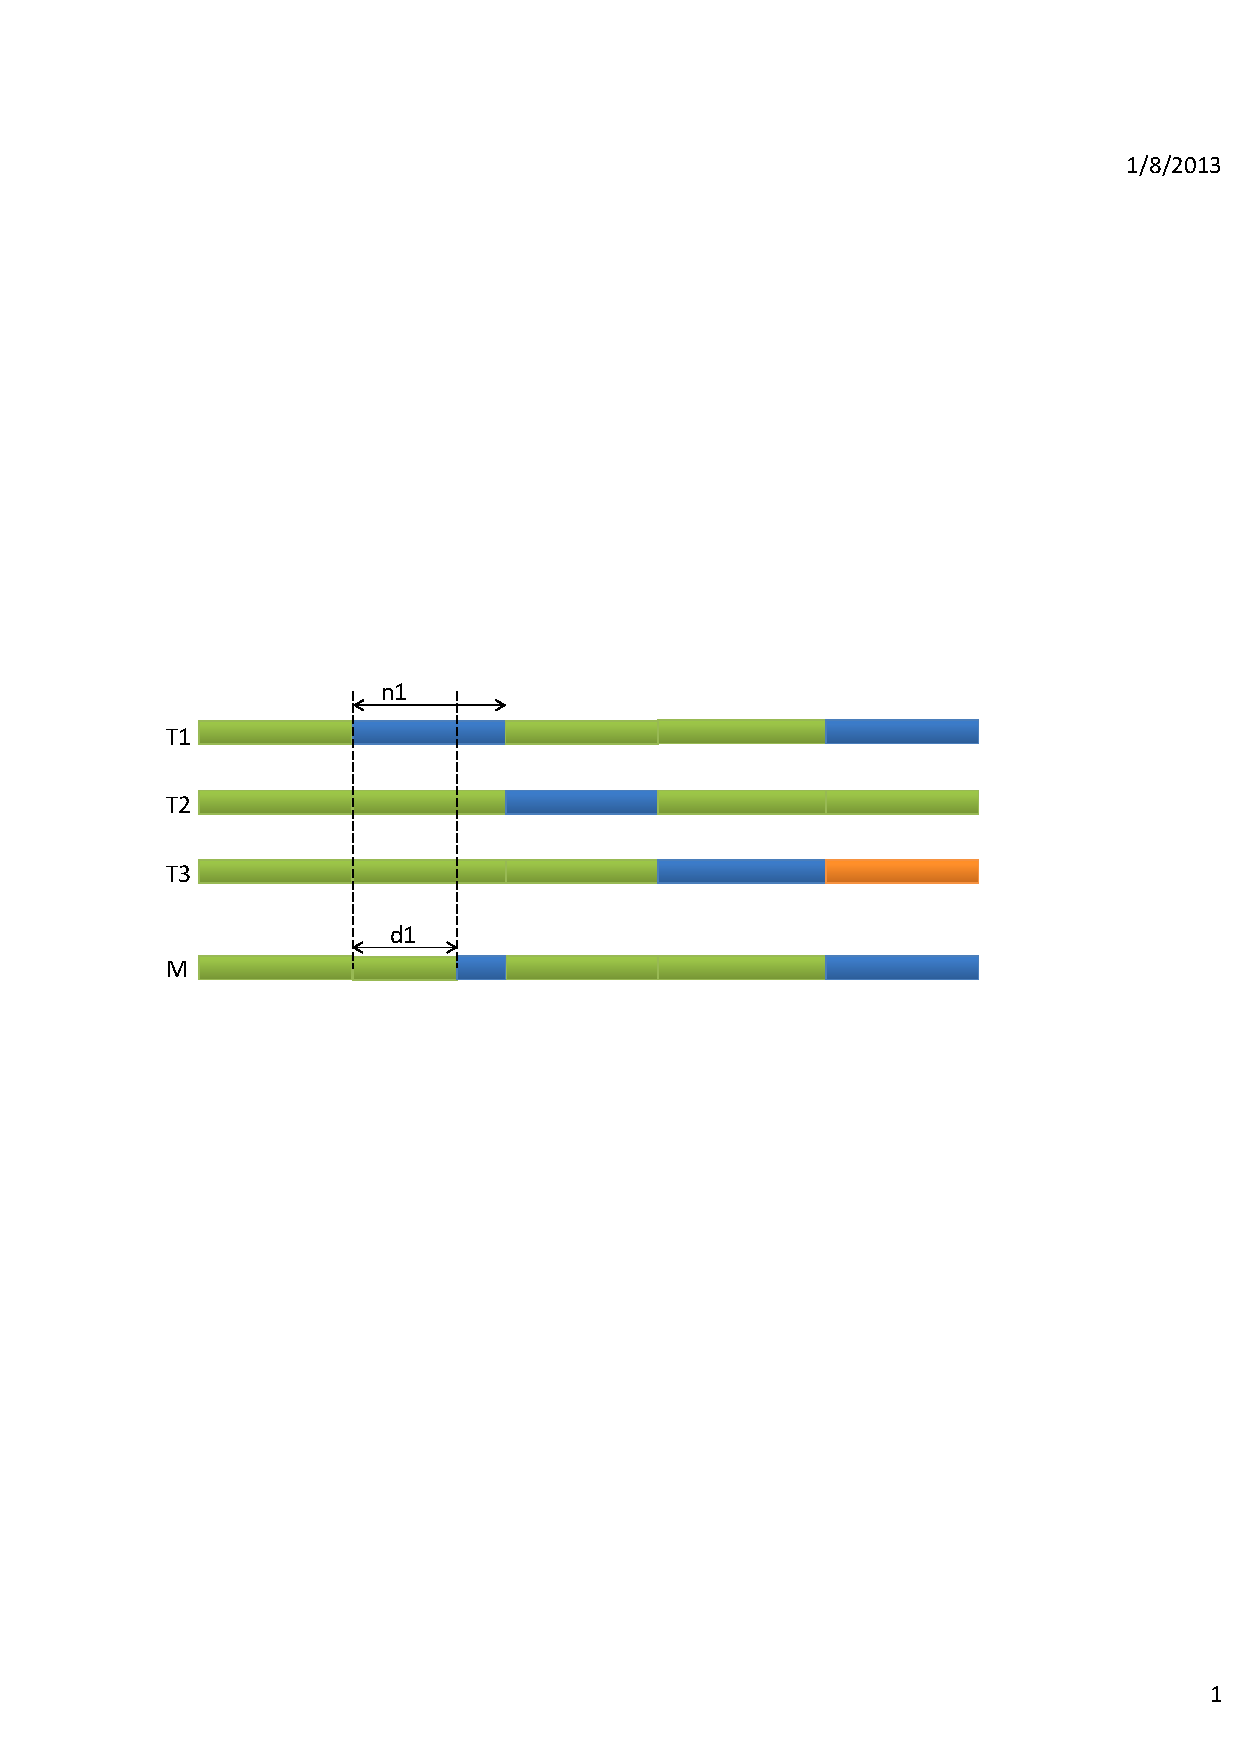
\includegraphics[width=\linewidth]{proof-case1}
Proof of theorem~\ref{th_3sufficient},  case 1:  There exists $i, 1 \leq i \leq 3$ for which $n_i\geq d_i$.
Without loss of generality we assume $i=1$.
The top 3 rows represent the input $l$-mers. The last row shows a common neighbor $M$. In any
column, identical colors represents matches, different colors represent mismatches.
\end{figure}

Case 2) For all $i, 1 \leq i \leq 3$ we have $n_i < d_i$. We construct $M$ as
shown in figure~\ref{figProofCase2}. For columns $k$ of type $N_0,N_2$ and $N_3$
we set $M[k]=t_1[k]$. For columns of type $N_1$ we set $M[k]=t_2[k]$.
For any $i,1\leq i \leq 3$ the following applies. If $n_i+n_4\leq d_i$ then the
Hamming distance between $M$ and $t_i$ is less than $d_i$ regardless of what
characters we choose for $M$ in the columns of type $N_4$.
On the other hand, if $n_i+n_4 > d_i$ then $M$ and $t_i$ have to match in at
least $n_i+n_4-d_i$ columns of type $N_4$. Thus, we pick
$max(0,n_i+n_4-d_i)$ columns of type $N_4$ and for each such column $k$ we set
$M[k]=t_i[k]$.
Now we prove that we actually have enough columns to make the
above choices, in other words $\Sigma_{i=1}^3max(0,n_i+n_4-d_i)\leq n_4$. This is equivalent to the following
conditions being true:
\begin{description}
\item[a)] For any $i, 1\leq i \leq 3$ we want $n_i+n_4-d_i \leq n_4$. This is
true because $n_i < d_i$.
\item[b)] For any $i,j, 1\leq i < j \leq 3$ we want
$(n_i+n_4-d_i)+(n_j+n_4-d_j) \leq n_4$. This can be rewritten as
$n_i+n_j+n_4\leq d_i+d_j$. The left hand side is $Hd(t_i, t_j)$ which
we know is less or equal to $d_i+d_j$.
\item[c)] We want $\Sigma_{i=1}^3n_i+n_4-d_i \leq n_4$. This can be rewritten as
$n_1 + n_2 + n_3 + 2 n_4 \leq d_1+d_2+d_3$. The left hand side is $Cd(T)$ which
we know is less than $d_1+d_2+d_3$.
\end{description}


\begin{figure}[!h]
\caption{Proof of theorem~\ref{th_3sufficient},
case 2}\label{figProofCase2}
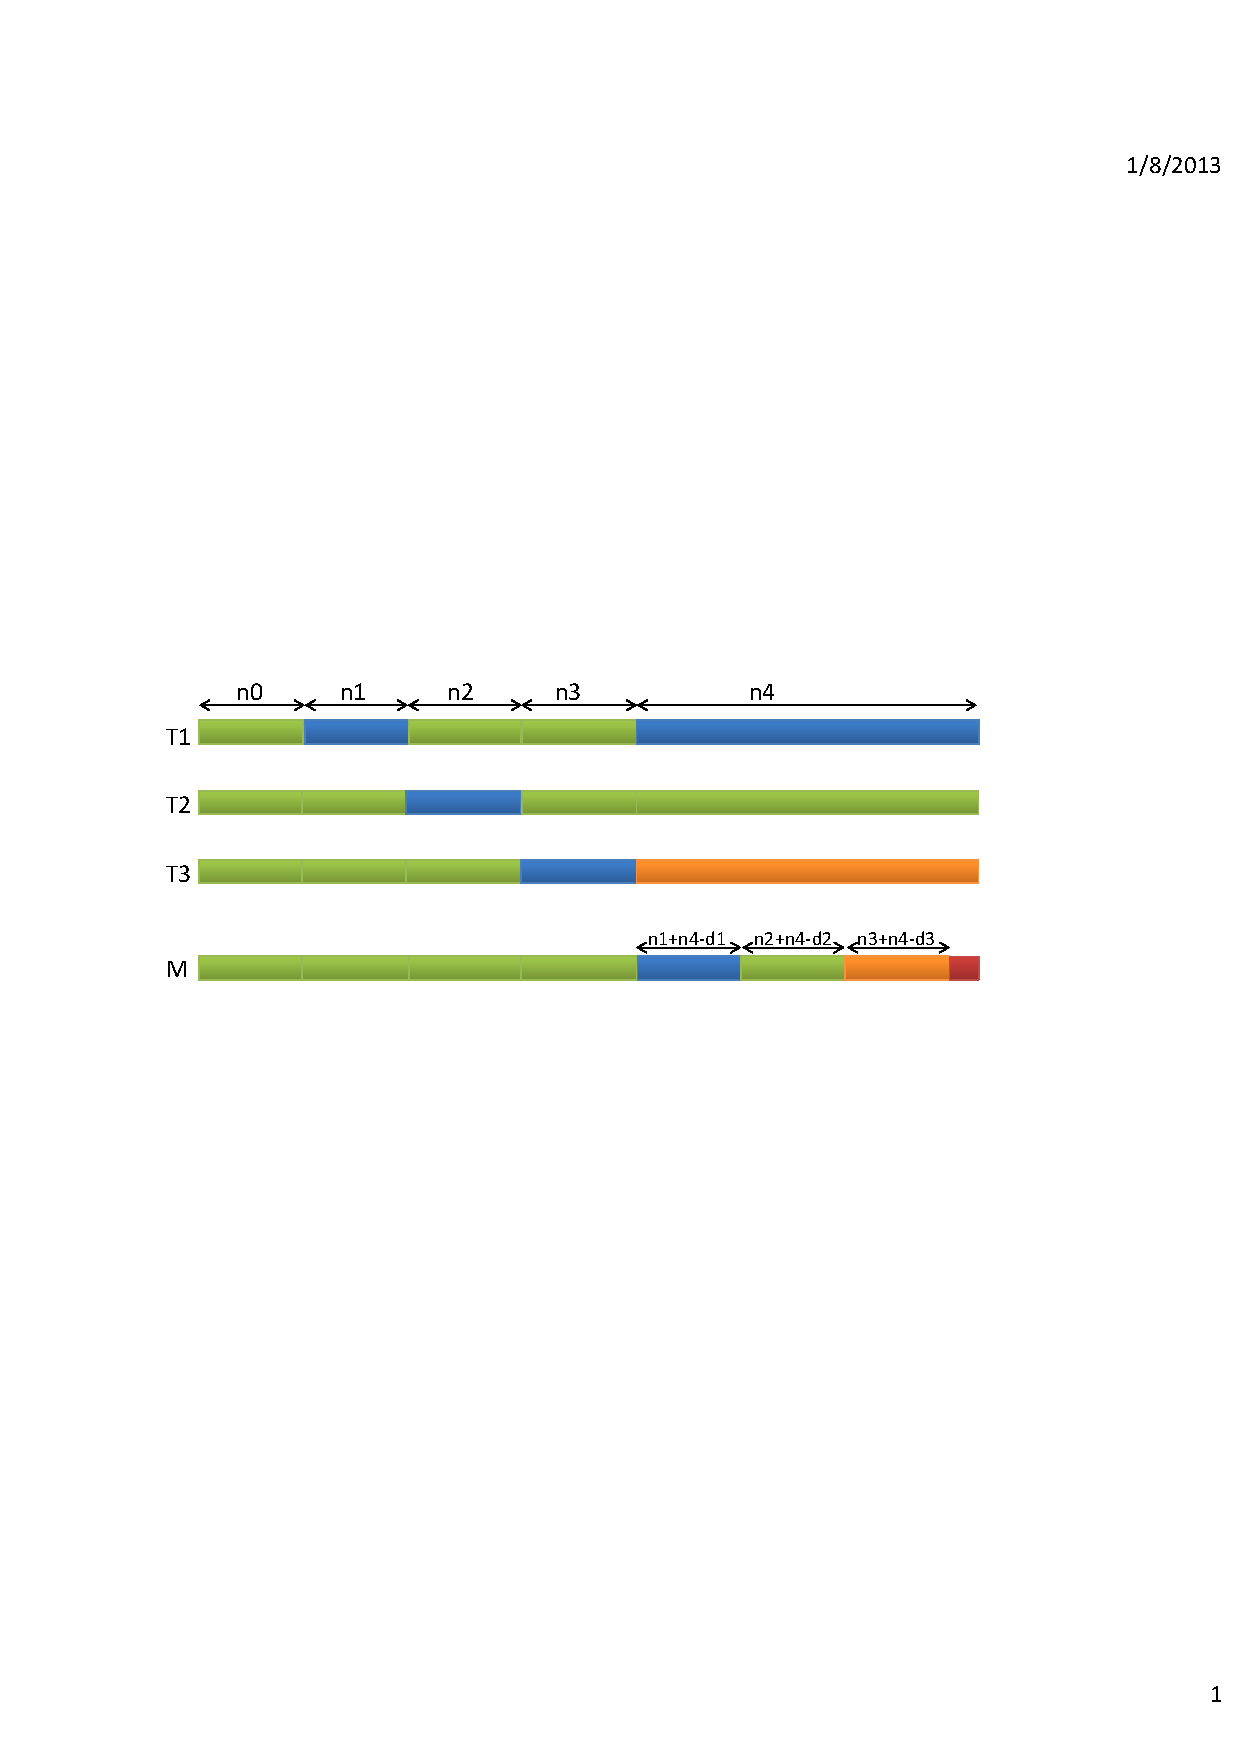
\includegraphics[width=\linewidth]{proof-case2}
Proof of theorem~\ref{th_3sufficient},
case 2: $n_i<d_i$ for all $i$, $1\leq i \leq 3$.
The top 3 rows represent the input $l$-mers. The last row shows a common neighbor $M$. In any
column, identical colors represents matches, different colors represent mismatches.
\end{figure}
\end{proof}



One of our reviewers kindly pointed out that the above proof is similar to an
algorithm in \cite{GNR01}.

\subsection{Adding Quorum Support}
In this section we extend the above techniques to solve the qPMS
problem. In the qPMS problem, when we generate tuples of $\ell$-mer, we may
``skip'' some of the strings.
This translates to the implementation as follows: in the PMS version we
successively try every alive $\ell$-mer in a given string by adding it to
the tuple $T$ and recursively calling the algorithm for the remaining strings.
For the qPMS version we have an additional step where, if the value of $q$
permits, we skip the current string and try $\ell$-mers
from the next string. At all times we keep track of how many strings we have
skipped. The pseudocode is given in algorithm \ref{figAlgQGenTuples}.
We invoke the algorithm as $QGenerateTuples(n-Q+1, \{\}, 0, k, R)$
where $Q=\lfloor\frac{qn}{100}\rfloor$ and $R$ contains all the $\ell$-mers in
all the strings.

\commentOut{
\begin{figure}
    \centering
    \includegraphics[width=1.0\textwidth]{algQGenTuples}
    \caption{This pseudocode generates tuples of $\ell$-mers that can potentially 
    have common neighbors, for the qPMS problem.\label{figAlgQGenTuples}}
\end{figure}
}

\begin{algorithm}
\SetKwInOut{Input}{Input}
\SetKwFunction{QGenerateTuples}{QGenerateTuples}
\SetKwFunction{ConsTotalDist}{Cd}
\SetKwFunction{GenerateNeighborhood}{GenerateNeighborhood}
\SetKwFunction{continue}{continue}

\caption{QGenerateTuples$(qTolerance,T,k,R)$} \label{figAlgQGenTuples}
\Input{$qTolerance$, number of strings we can afford to skip\;
\Indp\Indp $T=(t_1,t_2,\ldots,t_i)$, current tuple of $\ell$-mers\;
           $i$, last string processed\;
           $k$, desired size of the tuple\; 
           $R=(R_1, \ldots R_{n-i})$, where $R_j$ contains
           all alive $\ell$-mers in $s_{i+j}$\; 
}
\KwResult{Generates tuples of size $k$, containing $\ell$-mers, that have
common neighbors, then passes these tuples to the $\GenerateNeighborhood$
function\;}


\Begin{
\If {$|T|==k$}{
$\GenerateNeighborhood(T,d)$\;
\Return\;
}
outerLoop: \For {$u\in R_1$}{
$T':=T\cup \{u\}$\;
$incompat:=0$\; 
\For{$j \leftarrow 1$ \KwTo $n-i-1$}{
$R'_{j}=\{v \in R_{j+1} | \exists\; \text{common $d$-neighborhood for}\; T' \cup
\{v\}\}$\;
\If {$|R'_j|==0$} {
\If{$incompat \geq qTolerance$} {
\continue outerLoop\;
}
$incompat++$\;
}
$minAdd:=\min_{v \in R'_{j}} \ConsTotalDist(T'\cup \{v\}) -
\ConsTotalDist(T')$\; 
$aliveLmers:=|s_{i+j+1}|-|R'_{j}|$\; 
$sortKey[j]:= (minAdd, -aliveLmers)$ 
}
sort $R'$ decreasingly by $sortKey$\;
\QGenerateTuples$(qTolerance-incompat, T', k, R')$\;
}
\If{$qTolerance > 0$}{
\QGenerateTuples$(qTolerance-1, T, k, R \setminus R_1)$\;
}
}
\end{algorithm}


\subsection{Parallel Algorithm}

PMS8 and qPMS9 are parallel algorithms. Processor $0$ acts as both a master and
a worker, the other processors are workers. Each worker requests a subproblem from the
master, solves it, then repeats until all subproblems have been solved.
Communication between processors is done using the Message Passing Interface
(MPI). 

In PMS8, the subproblems are generated as follows. The search
space is split into $m=|s_1|-\ell+1$ independent subproblems $P_1, P_2,\ldots,
P_m$, where $P_i$ explores the $d$-neighborhood of $\ell$-mer $s_1[i..i+\ell-1]$.

In qPMS9, we extend the previous idea to the $q$ version. We split the
problem into subproblems $P_{1,1}, P_{1,2}, \ldots, P_{1,|s_1|-\ell+1}$,
$P_{2,1}, P_{2,2}, \ldots, P_{2,|s_2|-\ell+1}$, $\ldots$, $P_{r,1},
P_{r,2},\ldots,P_{r,|s_r|-\ell+1}$ where $r=n-Q+1$ and
$Q=\lfloor\frac{qn}{100}\rfloor$.
Problem $P_{i,j}$ explores the $d$-neighborhood of the $j$-th $\ell$-mer in string 
$s_i$ and searches for $\ell$-mers $M$ such that there are $Q-1$
instances of $M$ in strings $s_{i+1},\ldots,s_n$. Notice that $Q$ is
fixed, therefore subproblems $P_{i,j}$ get progressively easier as $i$
increases.


\subsection{Speedup Techniques}

\subsubsection{Speed up Hamming Distance calculation by packing $\ell$-mers}
\label{secCompressLmers}
By packing $\ell$-mers in advance we can speed up Hamming distance
operations. For example, we can pack 8 DNA characters in a 16 bit integer.
To compute the Hamming distance between two $l$-mers we first
perform an exclusive or of their packed representations. Equal
characters produce groups of zero bits, different characters produce
non-zero groups of bits.
For every possible $16$ bit integer $i$ we precompute the number of non-zero groups of bits
in $i$ and store it in a table. Therefore, one table look up provides the
Hamming distance for 8 DNA characters.  The same
technique applies to any alphabet $\Sigma$ besides DNA.

For an alphabet $\Sigma$ let $b=\lceil \log|\Sigma| \rceil$ be the number of
bits required to encode one character. Then, one compressed $\ell$-mer
requires $\ell * b$ bits of storage. However, due to
the overlapping nature of the $\ell$-mers in our input strings, we can employ
the following trick. In a 16 bit integer we can pack $p=\lfloor 16/b \rfloor$
characters. For every $\ell$-mer we only store the bit representation of its
first $p$ characters. The bit representation of the next $p$ characters is the
same as the bit representation of the first $p$ characters of the $l$-mer $p$ 
positions to the right of the current one. Therefore, the table of compressed
$l$-mers requires constant memory per $\ell$-mer, for a total of $O(n(m-l+1))$
words of memory.

\subsubsection{Preprocess Hamming distances for all pairs of input $\ell$-mers}
\label{secDistPairs}
The filtering step tests many times if two $l$-mers have a
distance of no more than $2d$. Thus, for every pair
of $l$-mers we preprocess this boolean information, provided the
required storage memory is not too high.

\subsubsection{Find motifs for a subset of the strings}
\label{secSubsetMotifs}
We also use the speedup technique described in \cite{RD11}: compute the motifs
for $n' < n$ of the input strings, then test each motif to see where it appears
in the remaining $n-n'$ strings. 

\subsubsection{Cache locality}
We can update $R$ in an efficient manner as follows. Every row in the
updated matrix $R'$ is a subset of the corresponding row in the current matrix
$R$, because some elements will be filtered out. Therefore, we can store $R'$
in the same memory locations as $R$. To do this, in each row, we move the elements belonging
to $R'$ at the beginning of the row and keep track of how many elements
belong to $R'$. To go from $R'$ back to $R$, we just have to restore the row
sizes to their previous values. The row elements will be the same even if they have
been permuted within the row. The same process can be repeated at every
step of the recursion, therefore the whole ``stack'' of $R$ matrices is stored in a
single matrix. This reduces the memory requirement and improves cache locality.
The cache locality is improved because at every step of the
recursion, in each row, we access a subset of the elements we accessed in the previous step, and
those elements are in contiguous locations of memory.


\subsection{Memory and Runtime}
Since we store all matrices $R$ in the space of a single matrix they
only require $O(n(m-l+1))$ words of memory. To this we add $O(n^2)$ words to store
 row sizes for the at most $n$ matrices which share the same space.
 The bits of information for $l$-mer pairs that have Hamming distance no
 more than $2d$ require $O((n(m-l+1))^2/w)$ words, where $w$ is the number of
 bits in a machine word.
The table of compressed $l$-mers takes $O(n(m-l+1))$ words. Therefore, the
total memory used by the algorithm is $O(n(n+m-l+1) + (n(m-l+1))^2 / w)$.

\subsection{Expected Number of Spurious Motifs}

It is useful to estimate how many ``spurious'' motifs (motifs expected by random
chance) will be found in a random sample. For that, we make the following
observations. The probability that a random $\ell$-mer $u$ is within distance
at most $d$ from another $\ell$-mer $v$ is

\begin{align}
p(\ell,d,\Sigma)=\frac{\sum_{i=0}^d\left(^\ell_i\right)(|\Sigma|-1)^i}{\Sigma^\ell}
\end{align}

The probability that an $\ell$-mer is within distance $d$ from any of the
$\ell$-mers in a string $S$ of length $m$ is: 

\begin{align}
P(m, \ell, d, \Sigma) = 1-(1-p(\ell,d,\Sigma))^{m-\ell+1}
\end{align}

The probability that an $\ell$-mer is within distance $d$ from at least
$q$ out of $n$ strings of length $m$ each is:

\begin{align}
Q(q,n,m,\ell,d,\Sigma)=\sum_{i=q}^n\left(^n_i\right)P(m,\ell,d,\Sigma)^i(1-P(m,\ell,d,\Sigma))^{n-i}
\end{align}

Therefore, the expected number of motifs for a given qPMS instance is:
$|\Sigma|^\ell Q(q,n,m,\ell,\Sigma)$. Based on
these formulas, we compute for every $\ell$ the largest value of $d$
such that the number of spurious motifs does not exceed 500. This gives us
the challenging instance for any $l$. These values are presented in table
\ref{maxdDNA} for DNA and table \ref{maxdProtein} for protein.

\section{Results}
\label{sec_pms_results}


As mentioned in the introduction, PMS algorithms are typically tested on
datasets generated as follows. 20 strings of length 600 each are generated from
the i.i.d. We choose an
$\ell$-mer $M$ as a motif and plant modified versions of it in $q\%$ of the
$n$ strings. Each planted instance is modified in $d$ random positions.
For every $(l,d)$ combination we generate 5 random datasets and report the
average runtime over all 5.

Programs were executed on the Hornet cluster at the University of Connecticut, 
which is a high-end, 104-node, 1408-core High Performance Computing cluster. 
For our experiments we used Intel Xeon X5650 Westmere cores. Results refer to
single core execution, unless specified otherwise.

\subsection{PMS8}
In this section we analyze the performance of PMS8 \cite{NRPMS14}.
The speedup obtained by the parallel version over the single core version,
for several challenging instances, is presented in figure~\ref{PMS8figSpeedup}.
The speedup for $p=48$ cores is close to $S=45$ and thus the
efficiency is $E=S/p=94\%$.

\begin{figure}
\caption{PMS8: Speedup of the multi-core version over the single core
version, for several datasets.}\label{PMS8figSpeedup} 
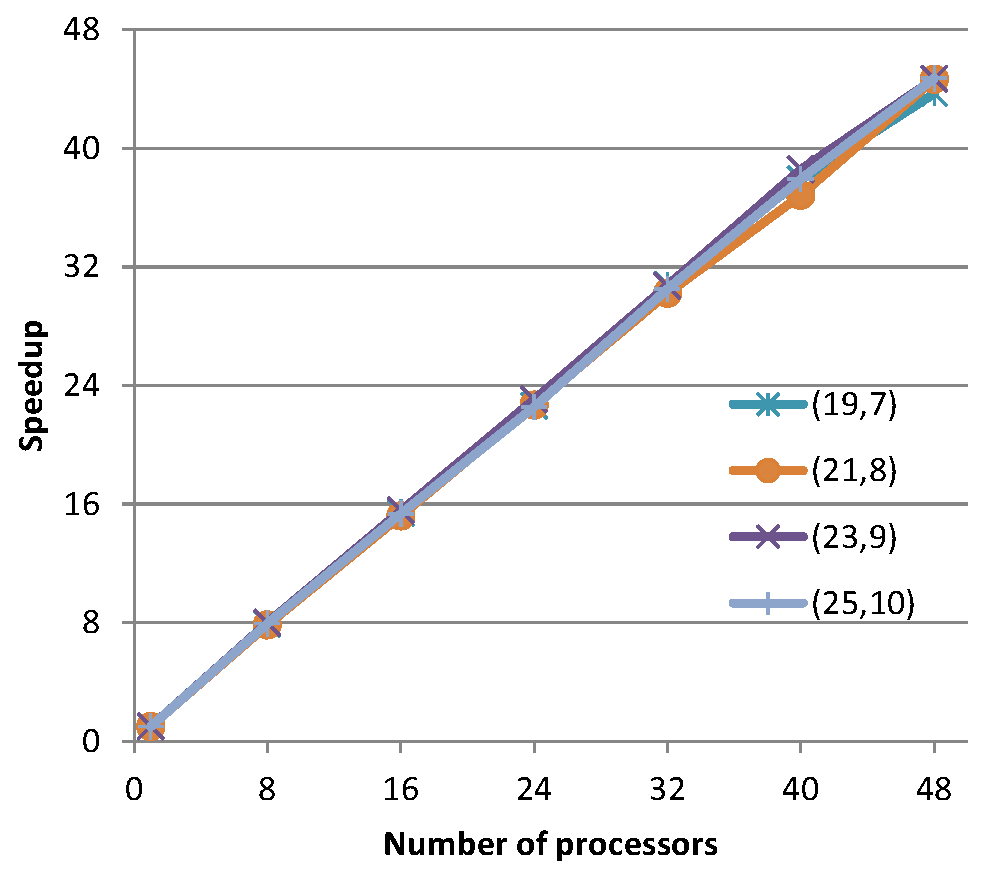
\includegraphics[width=\linewidth]{PMS8speedup}
\end{figure}

The runtime of PMS8 on instances with $l$ up to $50$ and $d$ up
to $21$ is shown in figure~\ref{PMS8figLDTable}. Instances which are expected to
have more than $500$ motifs simply by random chance (spurious motifs) are excluded.
Instances where $d$ is small relative to $l$ are solved using a single CPU core.
For more challenging instances we report the time taken using 48 cores.

\begin{figure}
\caption{PMS8: Runtimes for datasets with $l$ up to 50 and $d$ up to
25.}\label{PMS8figLDTable}
\includegraphics[width=1\linewidth]{PMS8dnaruntimes}
 All runtimes are averages over 5 random datasets.
 White background signifies single
core execution.  Blue background signifies execution using 48 cores.
Instances in gray have more than 500 spurious motifs. Orange
cells indicate unsolved instances. Time is reported in hours (h), minutes (m)
and seconds (s).
\end{figure}

A comparison between PMS8 and qPMS7 \cite{DRD12} on
challenging instances is shown in table~\ref{PMS8figCompChallenging}.
qPMS7 is a sequential algorithm. PMS8 was evaluated using up to 48 cores.
The speedup of PMS8 single core over qPMS7
is shown in figure~\ref{PMS8figSpeedupQPMS7}. The speedup is high for small
instances because qPMS7 has to load an ILP table. 
For larger instances the speedup of PMS8 sharply increases. This is expected
because qPMS7 always generates neighborhoods for tuples of $3$ $l$-mers, 
which become very large as $l$ and $d$ grow. On the other hand, PMS8 increases
the number of $l$-mers in the tuple with the instance size. 
 The peak memory used by qPMS7 for the challenging instances in
 table~\ref{PMS8figCompChallenging} was 607 MB whereas for PMS8 it was 122 MB.
 PMS8 was the first algorithm to solve the challenging instance (26,11).


\begin{table}
\caption{
 Comparison between qPMS7 and PMS8 on challenging instances. 
}\label{PMS8figCompChallenging}
\begin{tabular}{cccccc@{\extracolsep\fill}}
\hline
\textbf{Instance} & \textbf{qPMS7} & \textbf{PMS8$^1$} & \textbf{PMS8$^{16}$} &
\textbf{PMS8$^{32}$} & \textbf{PMS8$^{48}$} \\
\hline
(13,4) & 29s     & 7s     & 3s    & 2s    & 2s \\
(15,5) & 2.1m    & 48s    & 5s    & 4s    & 3s \\
(17,6) & 10.3m   & 5.2m   & 22s   & 12s   & 9s \\
(19,7) & 54.6m   & 26.6m  & 1.7m  & 52s   & 37s \\
(21,8) & 4.87h   & 1.64h  & 6.5m  & 3.3m  & 2.2m \\
(23,9) & 27.09h  & 5.48h  & 21.1m & 10.7m & 7.4m \\
(25,10)& -       & 15.45h & 1.01h & 30.4m & 20.7m \\
(26,11)& -       & -      & -     & -     & 46.9h \\
\hline
\end{tabular}\\
 PMS$8^P$ means  
 PMS8 used $P$ CPU cores. Both programs have been executed on the same hardware 
 and the same datasets. The times are average runtimes over 5 instances for each 
 dataset.
\end{table}



\begin{figure}
\caption{Speedup of PMS8 single core over qPMS7.}\label{PMS8figSpeedupQPMS7}
\includegraphics[width=\linewidth]{PMS8speedupQPMS7}
Ratio of runtimes between
qPMS7 and PMS8 running on a single core. Both programs have been executed on the same
hardware and the same datasets. The times are average runtimes over 5 instances
for each dataset.
\end{figure}


Some results in the literature have also focused on instances other than
the challenging ones presented above. A summary of these results and a comparison
with PMS8 is presented in table~\ref{pms8_table_comparison}. These results have been obtained on various types of hardware: single core,
multi-core, GPU, grid. In the comparison, we try to match the number of processors whenever possible.
The speed difference is of several orders of magnitude in some cases which indicates that
the pruning conditions employed by PMS8 significantly reduce the
search space compared to other algorithms.


\begin{table}

\caption{Comparison between PMS8 and contemporary
results in the literature.}\label{pms8_table_comparison}
\begin{tabular}{| p{2.5in} | p{0.5in} | p{0.5in} | p{0.6in} | p{0.4in} | p{0.4in} |}
\hline
Previous algorithm & Instance & Time & Cores & PMS8 Time & PMS8 Cores\\
\hline
Abbas et al. 2012 \cite{AAB12},  PHEP\_PMSprune & (21,8) & 20.42h & 8 & 6.5m & 1 \\
\hline
Yu et al. 2012 \cite{YHZG12}, PairMotif & (27, 9) & 10h & 1 & 4s & 1\\
\hline
\multirow{2}{*}{Desaraju and Mukkamala 2011 \cite{DeM11}} & (24,6) & 347s & 1 & 1s & 1\\
\cline{2-6}
                                         & (48,12)& 188s & 1 & 1s & 1\\
\hline
\multirow{2}{*}{\vbox{Dasari et al. 2011 \cite{DRZ11}, mSPELLER / gSPELLER}} & (21,8) & 3.7h & 16 & 6.5m & 16\\
\cline{2-6}
                                                   & (21,8) & 2.2h & \multirow{2}{*}{\vbox{4 GPUs x 240 cores}} & 6.5m & 16\\
\cline{1-3}\cline{5-6}
Dasari et al. 2010 \cite{DDZ10}, BitBased & (21,8) & 1.1h & & 6.5m & 16\\
\hline
Dasari and Desh 2010 \cite{DD10}, BitBased & (21,8) & 6.9h & 16 & 6.5m & 16\\
\hline
Sahoo et al. 2011 \cite{SSRP11} & (16,4) & 106s & 4 & 1s & 1\\
\hline
Sun et al. 2011 \cite{SLHTR11}, TreeMotif &(40,14) & 6h & 1 & 6s & 1\\
\hline
He et al. 2010 \cite{HLWR10}, ListMotif & (40,14) & 28,087s & 1 & 6s &1\\
\hline
Faheem 2010 \cite{Fah10}, skip-Brute Force & (15,4) & 2934s & 96 nodes & 1s & 1\\
\hline
\multirow{3}{*}{Ho et al. 2009 \cite{HJG09}, iTriplet} & (24,8) & 4h & 1 & 5s & 1\\
\cline{2-6}
                                      & (38,12) & 1h & 1 & 1s & 1\\
\cline{2-6}
                                      & (40,12) & 5m & 1 & 1s & 1\\
\hline
\end{tabular}\\
 Time is reported in seconds (s), minutes (m) 
or hours (h). Note that the hardware is different, though we tried to match
the number of processors when possible. Also, the instances are randomly
generated using the same algorithm, however the actual instances used by the
various papers are most likely different. For PMS8, the times are averages
over 5 randomly generated instances.
\end{table}



We compared PMS8 with qPMS7 on the real datasets discussed in
\cite{TLB+05}. We excluded datasets with less than $4$ input
sequences because these are not very challenging. For each dataset we chose two
combinations of $l$ and $d$. These combinations were chosen on a dataset
basis because for large values of $d$ the number of reported motifs is
excessive and for small values of $d$ the instance is not very challenging.
To make qPMS7 behave like PMS8 we set the quorum percent to $100\%$ ($q=n$).
The comparison is shown in table \ref{pms8_table_real_data}. Note that both algorithms
are exact algorithms and therefore the sensitivity and specificity are the same.


\begin{table}
\caption{Runtime comparison between PMS8 and qPMS7 on real datasets from
\cite{TLB+05}}\label{pms8_table_real_data}
\scalebox{0.96}{
\begin{tabular}{ccccccc@{\extracolsep\fill}}
\hline
\textbf{Dataset} & \textbf{n} & \textbf{Total no. bases} & \textbf{$\ell$} &
\textbf{d} & \textbf{PMS8 time} & \textbf{qPMS7 time}\\
\hline
dm01r & 4 & 6000 & 21 & 4 & 1 & 55 \\
dm01r & 4 & 6000 & 23 & 5 & 1 & 6 \\
dm04r & 4 & 8000 & 21 & 4 & 1 & 5 \\
dm04r & 4 & 8000 & 23 & 5 & 1 & 5 \\
\hline
hm01r & 18 & 36000 & 21 & 6 & 10 & 14 \\
hm01r & 18 & 36000 & 23 & 7 & 25 & 40 \\
hm02r & 9 & 9000 & 21 & 6 & 1 & 11 \\
hm02r & 9 & 9000 & 23 & 7 & 4 & 35 \\
hm03r & 10 & 15000 & 21 & 6 & 3 & 24 \\
hm03r & 10 & 15000 & 23 & 7 & 14 & 146 \\
hm04r & 13 & 26000 & 21 & 6 & 6 & 44 \\
hm04r & 13 & 26000 & 23 & 7 & 15 & 39 \\
hm05r & 3 & 3000 & 21 & 4 & 1 & 6 \\
hm05r & 3 & 3000 & 23 & 5 & 1 & 46 \\
hm08r & 15 & 7500 & 17 & 5 & 1 & 7 \\
hm08r & 15 & 7500 & 17 & 6 & 46 & 251 \\
hm19r & 5 & 2500 & 23 & 5 & 1 & 5 \\
hm19r & 5 & 2500 & 23 & 6 & 1 & 5 \\
hm20r & 35 & 70000 & 21 & 6 & 27 & 32 \\
hm20r & 35 & 70000 & 23 & 7 & 56 & 136 \\
hm26r & 9 & 9000 & 23 & 6 & 1 & 5 \\
hm26r & 9 & 9000 & 23 & 7 & 5 & 46 \\
\hline
mus02r & 9 & 9000 & 21 & 6 & 1 & 11 \\
mus02r & 9 & 9000 & 23 & 7 & 2 & 45 \\
mus04r & 7 & 7000 & 21 & 6 & 1 & 15 \\
mus04r & 7 & 7000 & 23 & 7 & 2 & 22 \\
mus05r & 4 & 2000 & 21 & 5 & 1 & 79 \\
mus05r & 4 & 2000 & 23 & 6 & 1 & 5 \\
mus07r & 4 & 6000 & 21 & 5 & 1 & 79 \\
mus07r & 4 & 6000 & 23 & 5 & 1 & 6 \\
mus10r & 13 & 13000 & 21 & 6 & 2 & 56 \\
mus10r & 13 & 13000 & 23 & 7 & 2 & 70 \\
mus11r & 12 & 6000 & 21 & 7 & 8 & 150 \\
mus11r & 12 & 6000 & 23 & 8 & 23 & 938 \\
\hline
yst01r & 9 & 9000 & 21 & 6 & 2 & 14 \\
yst01r & 9 & 9000 & 23 & 7 & 8 & 63 \\
yst02r & 4 & 2000 & 21 & 5 & 1 & 5 \\
yst02r & 4 & 2000 & 23 & 6 & 1 & 6 \\
yst03r & 8 & 4000 & 21 & 6 & 1 & 8 \\
yst03r & 8 & 4000 & 23 & 7 & 1 & 19 \\
yst04r & 6 & 6000 & 21 & 4 & 1 & 5 \\
yst04r & 6 & 6000 & 23 & 5 & 1 & 5 \\
yst05r & 3 & 1500 & 21 & 4 & 1 & 5 \\
yst05r & 3 & 1500 & 23 & 5 & 1 & 5 \\
yst06r & 7 & 3500 & 21 & 6 & 1 & 6 \\
yst06r & 7 & 3500 & 23 & 7 & 2 & 12 \\
yst08r & 11 & 11000 & 21 & 5 & 1 & 6 \\
yst08r & 11 & 11000 & 23 & 6 & 1 & 6 \\
yst09r & 16 & 16000 & 21 & 6 & 2 & 17 \\
yst09r & 16 & 16000 & 23 & 7 & 6 & 68 \\
\hline
\end{tabular}
}

For each dataset we tested two combinations of $l$ and $d$. For qPMS7 we set $q=n$. Both algorithms were executed on a single CPU core. Time is reported in seconds, rounded up to the next second.
\end{table}



\subsection{qPMS9}
In the previous section we have seen that PMS8 outperformed all of the
algorithms we could find in the literature at the time. After the
publication of PMS8, the TraverStringRef \cite{T14} algorithm came out.
Therefore, in this section we only compare PMS8, TraverStringRef and qPMS9. For
$q=100\%$ we compare all three algorithms, for $q=50\%$ we compare only the
algorithms that solve the quorum PMS problem: TraverStringRef and qPMS9.

For $q=100\%$, we compare the three algorithm on DNA data 
in table \ref{timePmsDna}. A similar comparison on protein data is given in
table \ref{timePmsProtein}.

For $q=50\%$, we compare TraverStringRef and
qPMS9 on DNA data in table \ref{timePmsDNAq50}. A similar comparison on protein
data is given in \ref{timePmsProteinq50}.

The running time of qPMS9 on DNA datasets for all combinations of $\ell$ and $d$
with $\ell$ up to 50 and $d$ up to 25, with $q=100\%$, is given in Figure
\ref{figDnaRuntimes}. The running time of qPMS9 on
protein datasets for all combinations of $\ell$ and $d$ with $\ell$ up to 30 and
$d$ up to 21, with $q=100\%$, is given in Figure \ref{figProteinRuntimes}.

\begin{figure}
    \caption{qPMS9 runtimes on DNA datasets for multiple combinations of $\ell$
    and $d$ where $q=100\%$. 
    \label{figDnaRuntimes}}
    \includegraphics[width=1.0\textwidth]{qpms9-dna-runtimes}
    The runtimes are averages over 5 random datasets. The
    times are given in hours (h) minutes (m) or seconds (s). Grey cells indicate instances that
    are expected to have more than 500 motifs by random chance (spurious
    motifs). Blue cells indicate that the program used 48 cores whereas white
    cells indicate single core execution. Instances in orange could not be
    solved efficiently.
\end{figure}

\begin{figure}
    \caption{qPMS9 runtimes on protein datasets for multiple combinations
    of $\ell$ and $d$ where $q=100\%$. }\label{figProteinRuntimes}
    \includegraphics[width=1.0\textwidth]{qpms9-protein-runtimes}
    The runtimes are averages over 5 random
    datasets. The times are given in hours (h) minutes (m) or seconds (s). 
    Grey cells indicate instances that
    are expected to have more than 500 motifs by random chance (spurious
    motifs). Blue cells indicate that the program used 48 cores whereas white
    cells indicate single core execution. Instances in orange could not be
    solved efficiently.
\end{figure}

\begin{table}
\caption{Maximum value of $d$ such
that the expected number of spurious motifs in random datasets does not exceed
$500$, for $\ell$ up to 50 and $q$ between $50\%$ and $100\%$, on DNA data.}\label{maxdDNA}
\begin{tabular}{| c | c | c | c |}
\hline
 & \multicolumn{3}{| c |}{max d}\\
\hline
L & $q=50\%$ & $q=75\%$ & $q=100\%$\\
\hline
13 & 3 & 3 & 4\\
14 & 3 & 4 & 4\\
15 & 4 & 4 & 5\\
16 & 4 & 5 & 5\\
17 & 4 & 5 & 6\\
18 & 5 & 6 & 6\\
19 & 5 & 6 & 7\\
20 & 6 & 7 & 7\\
21 & 6 & 7 & 8\\
22 & 7 & 8 & 8\\
23 & 7 & 8 & 9\\
24 & 8 & 9 & 9\\
25 & 8 & 9 & 10\\
26 & 9 & 10 & 11\\
27 & 9 & 10 & 11\\
28 & 10 & 11 & 12\\
29 & 10 & 11 & 12\\
30 & 11 & 12 & 13\\
31 & 11 & 12 & 13\\
32 & 12 & 13 & 14\\
33 & 12 & 13 & 14\\
34 & 13 & 14 & 15\\
35 & 13 & 15 & 16\\
36 & 14 & 15 & 16\\
37 & 14 & 16 & 17\\
38 & 15 & 16 & 17\\
39 & 15 & 17 & 18\\
40 & 16 & 17 & 18\\
41 & 16 & 18 & 19\\
42 & 17 & 18 & 20\\
43 & 17 & 19 & 20\\
44 & 18 & 19 & 21\\
45 & 18 & 20 & 21\\
46 & 19 & 21 & 22\\
47 & 19 & 21 & 22\\
48 & 20 & 22 & 23\\
49 & 20 & 22 & 24\\
50 & 21 & 23 & 24\\
\hline
\end{tabular}
\end{table}

\begin{table}
\caption{
Maximum value of $d$ such
that the expected number of spurious motifs in random datasets does not exceed
$500$, for $\ell$ up to 30 and $q$ between $50\%$ and $100\%$, on protein data.
}\label{maxdProtein}
\begin{tabular}{| c | c | c | c |}
\hline
 & \multicolumn{3}{| c |}{max d}\\
\hline
L & $q=50\%$  & $q=75\%$ & $q=100\%$ \\
\hline
9 & 4 & 4 & 5\\
10 & 4 & 5 & 5\\
11 & 5 & 6 & 6\\
12 & 6 & 6 & 7\\
13 & 6 & 7 & 8\\
14 & 7 & 8 & 8\\
15 & 8 & 9 & 9\\
16 & 9 & 9 & 10\\
17 & 9 & 10 & 11\\
18 & 10 & 11 & 11\\
19 & 11 & 12 & 12\\
20 & 11 & 12 & 13\\
21 & 12 & 13 & 14\\
22 & 13 & 14 & 15\\
23 & 14 & 15 & 15\\
24 & 14 & 15 & 16\\
25 & 15 & 16 & 17\\
26 & 16 & 17 & 18\\
27 & 16 & 18 & 19\\
28 & 17 & 18 & 19\\
29 & 18 & 19 & 20\\
30 & 19 & 20 & 21\\
\hline
\end{tabular}
\end{table}

\begin{table}
\caption{PMS runtimes for DNA data when $q=100\%$.}\label{timePmsDna}
\begin{tabular}{| c | c | c | c |}
\hline
$(\ell,d)$ & TraverStringRef & PMS8 &  qPMS9\\
\hline
(13,4) & 14s & 7s &  \textbf{6s}\\
\hline
(15,5) & 55s & 48s & \textbf{34s}\\
\hline
(17,6) & 3.5m & 5.2m & \textbf{2.7m}\\
\hline
(19,7) & 14.5m & 26.6m & \textbf{13.4m}\\
\hline
(21,8) & 59.8m & 1.64h & \textbf{45.4m}\\
\hline
(23,9) & 4.08h & 5.48h & \textbf{2.26h}\\
\hline
(25,10) & 17.55h & 15.45h & \textbf{6.3h}\\
\hline
\end{tabular}\\
 The time is given in
hours (h), minutes (m) or seconds (s), averaged over 5
datasets.
\end{table}

\begin{table}
\caption{PMS runtimes for protein data when $q=100\%$.}
\label{timePmsProtein}
\begin{tabular}{| c | c | c | c |}
\hline
$(\ell,d)$ & TraverStringRef & PMS8 & qPMS9\\
\hline
(10,5) & 2.6m & 42s & \textbf{37s}\\
\hline
(11,6) & 1.67h & 11m & \textbf{6.1m}\\
\hline
(13,7) & 58.2m & 2.6m & \textbf{19s}\\
\hline
(14,8) & TL & 1.03h & \textbf{29.6m}\\
\hline
(15,8) & 28.5m & 1.2m & \textbf{1.1m}\\
\hline
(17,9) & 16.6m & 45s & \textbf{43s}\\
\hline
(19,10) & 5.9m & \textbf{32s} & \textbf{32s}\\
\hline
(19,11) & TL & 1.23h & \textbf{30.1m}\\
\hline
(22,12) & 3.73h & 1.2m & \textbf{1.1m}\\
\hline
(24,13) & 1.84h & 48s & \textbf{47s}\\
\hline
(26,14) & 30.7m & \textbf{31s} & 32s\\
\hline
(26,15) & TL & 1.19h & \textbf{12.5m}\\
\hline
\end{tabular}\\
 The time is given in
hours (h), minutes (m) or seconds (s), averaged over 5
datasets. TL means that the program runs for more than 24h.
\end{table}


\begin{table}
\caption{
PMS runtimes for DNA data when $q=50\%$.}\label{timePmsDNAq50}
\begin{tabular}{| c | l | l |}
\hline
Instance & TraverStringRef & qPMS9\\
\hline
(20,6) & 3m & \textbf{1.5m}\\
\hline
(22,7) & 12.9m & \textbf{6.3m}\\
\hline
(23,7) & 2.6m & \textbf{48s}\\
\hline
(24,8) & 56m & \textbf{26.3m}\\
\hline
(25,8) & 9.9m & \textbf{3.1m}\\
\hline
(26,9) & 4.31h & \textbf{1.55h}\\
\hline
(27,9) & 39.9m & \textbf{10.6m}\\
\hline
(28,10) & 20.86h & \textbf{5.15h}\\
\hline
(29,10) & 2.89h & \textbf{34.5m}\\
\hline
\end{tabular}\\
 The time is given in
hours (h), minutes (m) or seconds (s), averaged over 5
datasets.
\end{table}


\begin{table}
\caption{
PMS runtimes for protein data when $q=50\%$.}
\label{timePmsProteinq50}
\begin{tabular}{| c | c | c | c |}
\hline
Instance & TraverStringRef & qPMS9\\
\hline
(9,4) & 11.3m & \textbf{3.7m}\\
\hline
(11,5) & 14m & \textbf{4.1m}\\
\hline
(12,6) & 6.22h & \textbf{57.5m}\\
\hline
(13,6) & 17.4m & \textbf{4.9m}\\
\hline
(14,7) & 5.09h & \textbf{41.3m}\\
\hline
(15,8) & TL & \textbf{4.62h}\\
\hline
(17,9) & TL & \textbf{1.79h}\\
\hline
(18,9) & 2.71h & \textbf{33.1m}\\
\hline
(20,10) & 2.33h & \textbf{33.3m}\\
\hline
(21,11) & TL & \textbf{50.9m}\\
\hline
\end{tabular}\\
 The time is given in
hours (h), minutes (m) or seconds (s), averaged over 5
datasets. TL means that the program runs for more than 24h.
\end{table}

\section{Discussion}
We have presented PMS8 and its successor qPMS9, which are efficient algorithms
for (Quorum) Planted Motif Search. PMS8 makes use of novel pruning
techniques for generating motif candidates. qPMS9 adds a new
procedure for exploring the search space and adds support for the quorum
version of PMS. qPMS9 is the first algorithm to solve the challenging DNA
instances $(28,12)$ and $(30,13)$. qPMS9 can
also efficiently solve instances with larger $\ell$ and $d$ such
as $(50,21)$ for DNA data or $(30,18)$ for protein data.

%For future work, one of our reviewers kindly pointed out that our approach of
%filtering $\ell$-mers for Hamming Distances could benefit for the work in
%\cite{PPB+08}.
